% -*- mode: LaTeX; compile-command: "./build.sh" -*-

\documentclass[xcolor={usenames,dvipsnames,svgnames,table},12pt]{beamer}

\mode<presentation>
{
  \usetheme{default}                          % use a default (plain) theme

  \setbeamertemplate{navigation symbols}{}    % don't show navigation
                                              % buttons along the
                                              % bottom
  \setbeamerfont{normal text}{family=\sffamily}

%  \setbeamertemplate{footline}[frame number]

  \AtBeginSection[]
  {
    \begin{frame}<beamer>
      \frametitle{}
      \begin{center}
        {\Huge \insertsectionhead}

        % \vspace{0.25in}
        % \includegraphics[width=2in]{\secimage}
      \end{center}
    \end{frame}
  }
}

\newenvironment{xframe}[1][]
  {\begin{frame}[fragile,environment=xframe,#1]}
  {\end{frame}}

% uncomment me to get 4 slides per page for printing
% \usepackage{pgfpages}
% \pgfpagesuselayout{4 on 1}[uspaper, border shrink=5mm]

% \setbeameroption{show only notes}

% \usepackage[english]{babel}
\usepackage[T1]{fontenc}
\usepackage{graphicx}
\graphicspath{{images/}}

\usepackage{ulem}
\usepackage{url}
\usepackage{fancyvrb}

\usepackage[backend=pgf, input, extension=pgf, outputdir=diagrams]{diagrams-latex}
\usepackage{sproof}

\usepackage{minted}


%%%%%%%%%%%%%%%%%%%%%%%%%%%%%%%%%%%%%%%%%%%%%%%%%%%%%%%%%%%%

\newcommand{\toB}{\mathit{toBinary}}
\newcommand{\fromB}{\mathit{fromBinary}}
\newcommand{\set}[1]{\mathit{set}\;{#1}}
\newcommand{\unset}[1]{\mathit{unset}\;{#1}}
\newcommand{\while}[2]{\mathit{while}\;{#1}\;{#2}}
\newcommand{\even}{\mathit{even}}
\newcommand{\odd}{\mathit{odd}}
\newcommand{\shl}{\mathit{shl}}
\newcommand{\shr}{\mathit{shr}}
\newcommand{\activeParent}{\mathit{activeParent}}

%%%%%%%%%%%%%%%%%%%%%%%%%%%%%%%%%%%%%%%%%%%%%%%%%%%%%%%%%%%%

% Todo: include picture of Fenwick tree on title slide

\title{You Could Have Invented Fenwick Trees!}
\date{
\includegraphics[height=0.25in]{plclub-logo_small} \\ 21 May 2021}
\author{Brent Yorgey}

%%%%%%%%%%%%%%%%%%%%%%%%%%%%%%%%%%%%%%%%%%%%%%%%%%%%%%%%%%%%%%%%%%%

\begin{document}

\maketitle

\begin{frame}{About me}
  \begin{center}
  \raisebox{-0.25\height}{
\includegraphics[height=0.25in]{plclub-logo_small}} (2008--2014) \\[0.25in]
  \raisebox{-0.25\height}{
\includegraphics[height=0.25in]{HENDRIX_LOGO_RGB}} (2015--) \\[0.25in]

  Things I Like (a very small sample):\\
  FP, EDSLs, combinatorics, category theory,
  teaching, competitive programming, questions from the audience
  \end{center}
\end{frame}

% \begin{frame}
%   \begin{center}
%     \includegraphics[width=2.5in,angle=-90]{noah-isaac}
%     \includegraphics[width=2.5in,angle=-90]{isaac-ruth}
%   \end{center}
% \end{frame}

% \begin{frame}{About this talk}
%   TODO: graph of git commits on this project
% \end{frame}

% TODO: drawArray a_1 ... a_8 as section image
% \def\secimage{array}
\section{Introduction}

\begin{xframe}{Sequence operations}
\begin{center}
\begin{diagram}[width=150]
import FenwickDiagrams

dia = vsep 0.5
  [ drawArray (draw . ("a_"++) . show) [1 :: Int .. 8]
  , mconcat
    [ arrowV unit_Y
    , text "update" # fontSizeL 0.5 # translate (1.5 ^& (-0.5))
    ]
    # translateX (3*leafWidth)
  , drawArray draw2 [1 :: Int .. 8]
  , rangeBracket 2 5
  , mconcat
    [ arrowV unit_Y
    , text "range query" # fontSizeL 0.5 # translate (2.2 ^& (-0.5))
    ]
    # translateX (2.5 * leafWidth)
  , text "$a_2 + a_3 + x + a_5$" # fontSizeL 0.6
    # translateX (2.5 * leafWidth)
  ]
  where
    draw2 4 = draw "x"
    draw2 n = draw ("a_" ++ show n)
\end{diagram}
\end{center}
\end{xframe}

% IFTIME: use colors for ranges instead of brackets
\begin{xframe}{Prefix queries}
\begin{center}
\begin{diagram}[width=150]
import FenwickDiagrams

dia = vsep 0.5
  [ drawArray draw (map (("a_"++) . show) [1 :: Int .. 8])
  , rangeBracket 3 6
  , text "=" # translateX (3.5 * leafWidth) <> strutY 1
  , drawArray draw (map (("a_"++) . show) [1 :: Int .. 8])
  , rangeBracket 1 6
  , text "-" # translateX (3.5 * leafWidth) <> strutY 1
  , drawArray draw (map (("a_"++) . show) [1 :: Int .. 8])
  , rangeBracket 1 2
  ]
  # fontSizeL 0.7
\end{diagram}
\end{center}
\end{xframe}

\begin{xframe}{Solutions}
  \begin{center}
  \begin{tabular}{ccc}
    approach & update & prefix query \\
    \onslide<2->{just store sequence} & $O(1)$ & $O(n)$ \\
    \onslide<3->{cache prefix sums}    & $O(n)$ & $O(1)$ \\
    \onslide<4->{cache more cleverly\dots?} & $O(\lg n)$ & $O(\lg n)$
  \end{tabular}
  \end{center}
\end{xframe}

\begin{xframe}{Segment trees}
\begin{center}
\begin{diagram}[width=300]
  import FenwickDiagrams
  import SegTree

  dia :: Diagram B
  dia = sampleArray
    # mkSegTree
    # fmap getSum
    # drawSegTree def
\end{diagram}

(assume $n = 2^k$)
\end{center}
\end{xframe}

\begin{xframe}{Updating a segment tree}
\begin{center}
\begin{diagram}[width=300]
  import FenwickDiagrams
  import SegTree
  import Data.Monoid
  import Control.Arrow ((***))

  dia :: Diagram B
  dia = sampleArray
    # map ((,) (Any False))
    # mkSegTree
    # update 5 (Any True, Sum 3)
    # fmap (getAny *** getSum)
    # drawSegTree (mkSTOpts showUpdateOpts)
\end{diagram}
\end{center}
\end{xframe}

\begin{xframe}{Range query on a segment tree}
\begin{center}
\begin{diagram}[width=300]
  import FenwickDiagrams
  import SegTree
  import Data.Monoid
  import Control.Arrow ((***), second)

  dia :: Diagram B
  dia = vsep 0.7
    [ sampleArray
      # mkSegTree
      # rq' i j
      # fst
      # drawSegTree (mkSTOpts showRangeOpts)
    , (fst (leafX i n) ^& 0) ~~ (snd (leafX j n) ^& 0)
      # lc green
      # applyStyle defRangeStyle
    ]
    where
      i = 4
      j = 11
      n = length sampleArray
\end{diagram}
\end{center}
\end{xframe}

% TODO: get rid of range bars in this diagram
\begin{xframe}{Thinning segment trees}
\begin{center}
\begin{diagram}[width=300]
  import FenwickDiagrams
  import SegTree
  import Data.Monoid
  import Control.Arrow ((***), first, second)

  dia :: Diagram B
  dia = sampleArray
    # mkSegTree
    # fmap getSum
    # drawSegTree def { drawNode = drawNode' def { rangeStyle = const (mempty # lw none) } }

\end{diagram}
\end{center}
\end{xframe}

\begin{xframe}{Thinning segment trees}
\begin{center}
\begin{diagram}[width=300]
  import FenwickDiagrams
  import SegTree
  import Data.Monoid
  import Control.Arrow ((***), first, second)

  dia :: Diagram B
  dia = sampleArray
    # mkSegTree
    # deactivate
    # drawSegTree (mkSTOpts (showInactiveOpts False))
\end{diagram}
\end{center}
\end{xframe}

% TODO: picture showing how any prefix corresponds to a specific
% collection of active nodes?

\begin{xframe}{Storing a thinned segment tree}
\begin{center}
\begin{diagram}[width=300]
  import FenwickDiagrams
  import SegTree
  import Data.Monoid
  import Control.Arrow ((***), first, second)

  dia :: Diagram B
  dia = vsep 0.5
    [ sampleArray
      # mkSegTree
      # deactivate
      # drawSegTree opts
    , arrowV (2 *^ unit_Y)
    , sampleArray
    # mkFenwickArray
    # drawArray (draw . getSum)
    # centerX
    ]

  opts = (mkSTOpts (showInactiveOpts False))
    { drawEdge = drawSlidingEdges }
\end{diagram}
\end{center}
\end{xframe}

\begin{xframe}{Fenwick tree = right-leaning, thinned segment tree}
  \begin{center}
\begin{diagram}[width=300]
{-# LANGUAGE LambdaCase #-}
import FenwickDiagrams
import SegTree

dia :: Diagram B
dia = sampleArray
  # mkSegTree
  # deactivate
  # drawSegTree stOpts

stOpts = (mkSTOpts nOpts)
  { leanRight = True }

nOpts = (showInactiveOpts False)
  { leanRightN = True
  , rangeStyle = \case { (_, Active) -> defRangeStyle; _ -> mempty # lw none }
  }
\end{diagram}

\onslide<2>{\dots but how to move around?}
  \end{center}
\end{xframe}

\begin{xframe}{Fenwick trees}
  \begin{center}
    \begin{minipage}{0.45\textwidth}
      \raisebox{-0.5\height}{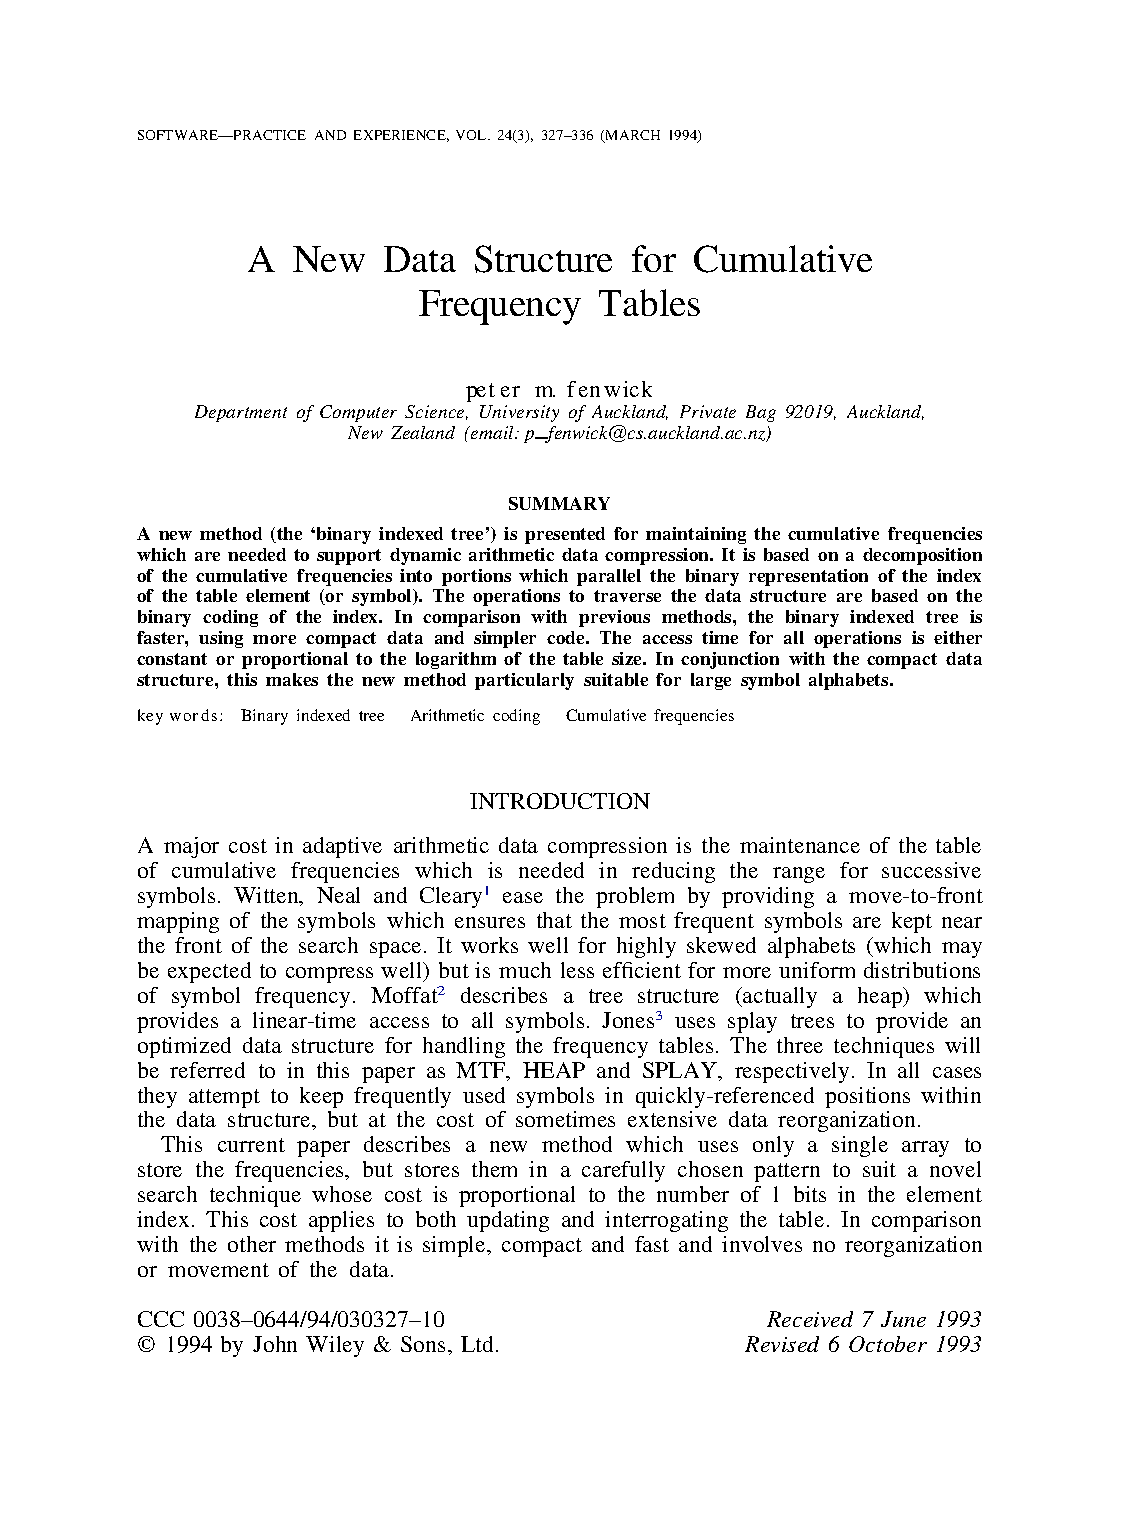
\includegraphics[height=3in]{fenwick-p1}}
    \end{minipage}
    \hspace{0.25in}
    \begin{minipage}{0.45\textwidth}
      Peter Fenwick, 1994 \\
      A New Data Structure for Cumulative Frequency Tables
    \end{minipage}
  \end{center}
  % IFTIME show Ryabko paper too
\end{xframe}

\begin{xframe}{Implementing Fenwick trees}
  \inputminted[fontsize=\footnotesize]{java}{FenwickTree.java}
\end{xframe}

% IF TIME, show why this definition of LSB works.
% Otherwise leave it as exercise.  2's complement, to negate we flip
% all the bits then increment.  This means -x has all opposite bits as
% x up to the LSB, then is the same from the LSB onwards.

\begin{xframe}{LSB = Least Significant Bit}
  \[ \mathrm{LSB}(01101100) = 00000100 \]
  \bigskip

  \onslide<2->{
    $\mathrm{LSB}(x) = x \mathbin{\&} (-x)$?  Hint: in 2's complement,
    $(-x) = \overline{x} + 1$.
  }
\end{xframe}

\section{Indexing trees}

\begin{xframe}{Indexing full binary trees}
  \begin{center}
  \begin{diagram}[width=250]
import Diagrams.Prelude hiding (Empty)
import Diagrams.TwoD.Layout.Tree
import Data.Maybe (fromJust)

-- bt depth root
bt :: Int -> Int -> BTree Int
bt 0 _ = Empty
bt d r = BNode r (bt (d-1) (2*r)) (bt (d-1) (2*r+1))

dia = bt 4 1
  # symmLayoutBin' (with & slHSep .~ 4 & slVSep .~ 4)
  # fromJust
  # renderTree dn (~~)

dn i = text ("$" ++ show i ++ "$") <> circle 1 # fc white
  \end{diagram}
  \end{center}
\end{xframe}

\begin{xframe}{Indexing full binary trees, in binary}
  \begin{center}
  \begin{diagram}[width=250]
import Diagrams.Prelude hiding (Empty)
import Diagrams.TwoD.Layout.Tree
import Data.Maybe (fromJust)
import Numeric

-- bt depth root
bt :: Int -> Int -> BTree Int
bt 0 _ = Empty
bt d r = BNode r (bt (d-1) (2*r)) (bt (d-1) (2*r+1))

dia = bt 4 1
  # symmLayoutBin' (with & slHSep .~ 4 & slVSep .~ 4)
  # fromJust
  # renderTree dn (~~)
  # fontSizeL 0.8

dn i = text ("$" ++ showIntAtBase 2 ("01"!!) i "" ++ "$") <> circle 1 # fc white # lw none
  \end{diagram}
  \end{center}
\end{xframe}

\begin{xframe}{The Plan}
  \begin{itemize}
  \item Derive Fenwick tree $\leftrightarrow$ binary
    tree index conversion
  \item Compute motion through a Fenwick tree (array) as $\fromB
    \circ \mathit{binaryMotion} \circ \toB$
  \item Fuse
  \item Profit!
  \end{itemize}
\end{xframe}

\begin{xframe}{Fenwick $\to$ binary}
  \begin{center}
  \begin{diagram}[width=250]
import Diagrams.Prelude hiding (Empty)
import Diagrams.TwoD.Layout.Tree
import Data.Maybe (fromJust)
import Control.Monad.State

-- bt depth root left?
bt :: Int -> Int -> Bool -> State Int (BTree (Int, Maybe Int))
bt 0 _ _ = return Empty
bt d r left = do
  lt <- bt (d-1) (2*r) True
  rt <- bt (d-1) (2*r+1) False
  l <- get
  when left (modify (+1))
  return (BNode (r, if left then Just l else Nothing) lt rt)

dia = evalState (bt 4 1 True) 1
  # symmLayoutBin' (with & slHSep .~ 4 & slVSep .~ 4)
  # fromJust
  # renderTree dn (~~)

dn :: (Int, Maybe Int) -> Diagram B
dn (i,ml) = mconcat
  [ text ("$" ++ show i ++ "$") # translateX (-0.7)
  , vrule 3
  , circle 1.5
  , case ml of
      Nothing -> arc' 1.5 (direction unit_Y) ((1/2) @@ turn)
                 # closeTrail # strokeT # translateY (-1.5)
                 # fc grey # lw none
      Just l  -> text ("$" ++ show l ++ "$") # fc blue # translateX 0.7
                 # fontSizeL 0.9
  , circle 1.5 # fc white # lw none
  ]
  # fontSizeL 0.7
  \end{diagram}
  \vspace{0.25in}

  \begin{tabular}{cccccccc}
    \textcolor{blue}{1} & \textcolor{blue}{2} & \textcolor{blue}{3}  & \textcolor{blue}{4} & \textcolor{blue}{5} & \textcolor{blue}{6} & \textcolor{blue}{7} & \textcolor{blue}{8} \\
    8 & 4 & 10 & 2 & 12 & 6 & 14 & 1
  \end{tabular}
  \end{center}

\end{xframe}

\begin{xframe}{Fenwick $\to$ binary}
  \begin{center}
  \begin{diagram}[width=300]
import Diagrams.Prelude hiding (Empty)
import Diagrams.TwoD.Layout.Tree
import Data.Maybe (fromJust)
import Control.Monad.State

-- bt depth root left?
bt :: Int -> Int -> Bool -> State Int (BTree (Int, Maybe Int))
bt 0 _ _ = return Empty
bt d r left = do
  lt <- bt (d-1) (2*r) True
  rt <- bt (d-1) (2*r+1) False
  l <- get
  when left (modify (+1))
  return (BNode (r, if left then Just l else Nothing) lt rt)

dia = evalState (bt 5 1 True) 1
  # symmLayoutBin' (with & slHSep .~ 4 & slVSep .~ 4)
  # fromJust
  # renderTree dn (~~)

dn :: (Int, Maybe Int) -> Diagram B
dn (i,ml) = mconcat
  [ text ("$" ++ show i ++ "$") # translateX (-0.7)
  , vrule 3
  , circle 1.5
  , case ml of
      Nothing -> arc' 1.5 (direction unit_Y) ((1/2) @@ turn)
                 # closeTrail # strokeT # translateY (-1.5)
                 # fc grey # lw none
      Just l  -> text ("$" ++ show l ++ "$") # fc blue # translateX 0.7
                 # fontSizeL 0.9
  , circle 1.5 # fc white # lw none
  ]
  # fontSizeL 0.7
  \end{diagram}
  \vspace{0.25in}

  \begingroup
  \setlength{\tabcolsep}{4pt}
  \begin{tabular}{cccccccccccccccc}
    \textcolor{blue}{1} & \textcolor{blue}{2} & \textcolor{blue}{3}  & \textcolor{blue}{4} & \textcolor{blue}{5} & \textcolor{blue}{6} & \textcolor{blue}{7} & \textcolor{blue}{8} & \textcolor{blue}{9} & \textcolor{blue}{10} & \textcolor{blue}{11} & \textcolor{blue}{12} & \textcolor{blue}{13} & \textcolor{blue}{14} & \textcolor{blue}{15} & \textcolor{blue}{16} \\
    16 & \textcolor{green}{8} & 18 & \textcolor{green}{4} & 20 & \textcolor{green}{10}
     & 22 & \textcolor{green}{2} & 24 & \textcolor{green}{12} & 26 & \textcolor{green}{6} & 28 & \textcolor{green}{14} & 30 & \textcolor{green}{1}
  \end{tabular}
  \endgroup
  \end{center}

\end{xframe}

\newcommand{\merge}{\curlyvee}
\begin{xframe}{toBinary}
  \begin{align*}
    [] \merge \_ &= [] \\
    (x::xs) \merge ys &= x :: (ys \merge xs) \\ \\
    s_0 &= [1] \\
    s_n &= [2^n, 2^n + 2, \dots, 2^{n+1}-2] \merge s_{n-1} \\ \\
    \toB_n(k) &= s_n\;!\;k \qquad \text{(1-indexed)}
  \end{align*}
\end{xframe}

\begin{xframe}{Interleaving lemmas}
  \begin{align*}
    (xs \merge ys)\; ! \; 2k &= ys\;!\;k \\
    (xs \merge ys)\; ! \; (2k - 1) &= xs\;!\;k
  \end{align*}
\end{xframe}

\begin{xframe}{Simplifying toBinary}
  \begin{align*}
    s_0 &= [1] \\
    s_n &= [2^n, 2^n + 2, \dots, 2^{n+1}-2] \merge s_{n-1} \\ \\
    toBinary_n(2k)   &= s_n\;!\;2k = s_{n-1}\;!\;k \\
    toBinary_n(2k-1) &= [2^n, 2^n + 2, \dots]\;!\; k = 2^n + 2(k-1)
  \end{align*}
  \onslide<2->{
    \[ \toB_n(j) = \begin{cases}
        \toB_{n-1}(j/2) & \text{$j$ even} \\ 2^n + j - 1
        & \text{$j$ odd} \end{cases} \]
  } \bigskip
\end{xframe}

\begin{xframe}{Simplifying toBinary}
    \[ \toB_n(j) = \begin{cases}
        \toB_{n-1}(j/2) & \text{$j$ even} \\ 2^n + j - 1
        & \text{$j$ odd} \end{cases} \] \bigskip

  Let $k = 2^a b$ where $b$ is odd.  Then
  \[ \toB_n(2^a b) = \toB_{n-a}(b) =
    2^{n-a} + b - 1. \]
\end{xframe}

\begin{xframe}{toBinary as bit operations?}
  \[ \toB_n(2^a b) = 2^{n-a} + b - 1 \]

  Given $k = 2^a b < 2^n$ ($2^n \to 1$ is special case):
  \begin{itemize}
  \item set $2^n$ bit ($2^n + 2^a b$)
  \item shift right until final bit is $1$  ($2^{n-a} + b$)
  \item set final bit to $0$ ($2^{n-a} + b - 1$)
  \end{itemize} \medskip

  \[ \toB_n = \unset 0 \circ \while{\even}{\shr} \circ
    \set{n} \]

  \onslide<2->{Question: what is the right DSL for expressing this bit
    manipulation procedure?}

    % TODO: express this using a little bit DSL
\end{xframe}

\begin{xframe}{fromBinary}
  \[ \toB_n = \unset 0 \circ \while{\even}{\shr} \circ
    \set{n} \]

  $\fromB_n$ ($1 \to 2^n$ is special case):
  \begin{itemize}
  \item set final bit to $1$
  \item shift left until MSB is $2^n$
  \item set $2^n$ bit to 0
  \end{itemize} \medskip

  \[ \fromB_n = \unset n \circ \while{(< 2^n)}{\shl} \circ \set 0 \]
\end{xframe}

\begin{xframe}{$\fromB_n \circ \toB_n$ example}
  \begin{sproof}
    \stmt{00110100}
    \reason{\to}{$\set n$}
    \stmt{10110100}
    \reason{\to}{$\while{\even}{\shr}$}
    \stmt{00101101}
    \reason{\to}{$\unset 0$}
    \stmt{00101100}
    \reason{\to}{$\set 0$}
    \stmt{00101101}
    \reason{\to}{$\while{(< 2^n)}{\shl}$}
    \stmt{10110100}
    \reason{\to}{$\unset n$}
    \stmt{00110100}
  \end{sproof}
\end{xframe}

\begin{xframe}{Update}
  \begin{center}
\begin{diagram}[width=300]
import Diagrams.Prelude hiding (Empty)
import Diagrams.TwoD.Layout.Tree
import Data.Maybe (fromJust)
import Control.Monad.State

-- bt depth root left?
bt :: Int -> Int -> Bool -> State Int (BTree (Int, Maybe Int))
bt 0 _ _ = return Empty
bt d r left = do
  lt <- bt (d-1) (2*r) True
  rt <- bt (d-1) (2*r+1) False
  l <- get
  when left (modify (+1))
  return (BNode (r, if left then Just l else Nothing) lt rt)

dia = evalState (bt 5 1 True) 1
  # symmLayoutBin' (with & slHSep .~ 4 & slVSep .~ 4)
  # fromJust
  # renderTree dn (~~)

dn :: (Int, Maybe Int) -> Diagram B
dn (i,ml) = mconcat
  [ text ("$" ++ show i ++ "$") # translateX (-0.7)
  , vrule 3
  , circle 1.5
  , case ml of
      Nothing -> arc' 1.5 (direction unit_Y) ((1/2) @@ turn)
                 # closeTrail # strokeT # translateY (-1.5)
                 # fc grey # lw none
      Just l  -> text ("$" ++ show l ++ "$") # fc blue # translateX 0.7
                 # fontSizeL 0.9
  , circle 1.5 # fc (case ml of { Just 6 -> lgr ; Just 8 -> lgr ; _ -> white })
               # lw none
  ]
  # fontSizeL 0.7
  where
    lgr = lightgreen
\end{diagram}

\onslide<2->{
  \[ \activeParent = \while{\odd}{\shr} \circ \shr \]
}
\end{center}
\end{xframe}

\begin{xframe}{Update}
  \begin{align*}
    \mathit{nextUpdate_n}
    &= \fromB_n \circ \activeParent \circ \toB_n \\
    &= \unset n \circ \while{(< 2^n)}{\shl} \circ \set 0 \\
    &\qquad\circ \while{\odd}{\shr} \circ \shr \\
    &\qquad\circ \unset 0 \circ \while{\even}{\shr} \circ \set{n} \\
    &= \unset n \circ \while{(< 2^n)}{\shl} \\
    &\qquad\circ \set 0 \circ \while{\odd}{\shr} \circ
      \while{\even}{\shr} \\
    &\qquad\circ \set{n} \\
    &= \dots \; ? \; \dots \\
    &= \lambda x. x + \mathit{LSB}\;x
  \end{align*}
\end{xframe}

\begin{xframe}{Update example}
  \begin{sproof}
    \stmt{00110}
    \reason{\to}{$\set n$}
    \stmt{10110}
    \reason{\to}{$\while{\even}{\shr}$}
    \stmt{01011}
    \reason{\to}{$\while{\odd}{\shr}$}
    \stmt{00010}
    \reason{\to}{$\set 0$}
    \stmt{00011}
    \reason{\to}{$\while{(< 2^n)}{\shl}$}
    \stmt{11000}
    \reason{\to}{$\unset n$}
    \stmt{01000}
  \end{sproof}
\end{xframe}

\begin{xframe}{}
  \begin{center}
    Thanks!
  \end{center}
\end{xframe}

\end{document}
